\section{Diseño y Arquitectura}
GeoDengue está basada en una arquitectura, de tres capas, cliente-servidor, en el que las tareas
se reparten entre los proveedores de recursos o servicios, denominados servidores, y los
demandantes, llamados clientes. La primera capa, la de presentación, es la que se encarga de
interactuar con el usuario final, la segunda capa es la de negocios, esta se encarga de procesar
las solicitudes realizadas por la capa de presentación y definir las reglas que deben aplicase en
para cada solicitud. Por último, se encuentra la capa de datos, donde se almacenan los datos,
porcesan las peticiones de la capa de negocios para persistir o recuperar información.

\begin{figure}
\centering
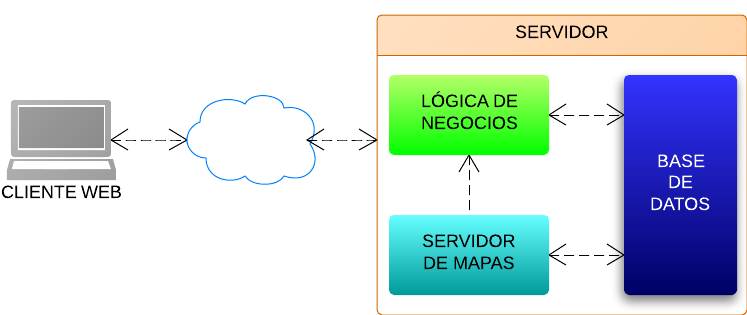
\includegraphics[width=0.9\textwidth]{capitulo-5/graphics/arquitectura-completa.png}
\caption{\label{fig:arquitectura-completa}Arquitectura de interacción de componentes de GeoDengue.}
\end{figure}

Se optó por un enfoque web debido a la practicidad de estas aplicaciones, el usuario final solo
debe contar con un navegador web. Estas deberían funcionar igual independientemente de la versión
del sistema operativo instalado en el cliente. Las aplicaciones web son catalogadas como
aplicaciones de bajo consumo, debido a que la mayor parte de la aplicación no se encuentra en
nuestro ordenador, y muchas de las tareas de procesamiento que realiza el software no consumen
recursos nuestros porque se realizan en el servidor.

La capa de presentación se encuentra diseñada como un Single Page Application o SPA (en español
Aplicación de una sola página). Un SPA es una aplicación que se ejecuta en una única página, donde
la navegación se realiza mediante cargas parciales, sin recargar el sitio completamente. La
comunicación con el servidor se realiza mendiante peticiones Ajax, para ello se cuenta con una
arquitectura basada en servicios REST.

